\documentclass{article}
\usepackage[utf8]{inputenc}
\usepackage{geometry}
\usepackage{graphicx}
\usepackage{pgfplots}
\usepackage{amsmath}
\usepackage{amssymb}
\usepackage{amsfonts}
\usepackage{mdframed}
\usepackage{amsthm}
\usepackage{physics}
\usepackage{derivative}
\usepackage{hyperref}
\usepackage{wrapfig}
\renewcommand{\theenumi}{\roman{enumi}}

\geometry{a4paper, left=2cm, right=2cm, top=1cm, bottom=2cm}

\pgfplotsset{compat=1.18}
\begin{document}

\begin{minipage}{0.7\textwidth}
    \small \textbf{Laboratorio de Electromagnetismo}  \\
    \small {Facultad de Ciencias, Universidad Nacional Autónoma de México} \\
    \small {Profesor: Eugenia Paola Arévalo López} \\
    \small {Ayudante: Luis Andrés Gómez González}\\
    \small {Fecha de entrega: 4 de Noviembre de 2024} \\
    \small {Nombre completo: Andrés López González} \\
    \small {Resumen de conferencia}
\end{minipage}
\hfill
\begin{minipage}{0.12\textwidth}
    
\includegraphics[width=\linewidth]{logo_universidad}
\end{minipage}

\section*{Explorando el Cosmos con Inteligencia Artificial}
\textbf{Conferencia impartida por el Dr. Octavio Valenzuela en el Instituto de Astronomía de la UNAM}
Auditorio Paris Pişmiş a 18/10/24 18:00hrs

\textit{El Dr. Valenzuela, investigador del IA-UNAM, es experto en galaxias, cosmología astrofísica y computacional. Ha abordado temas cruciales de materia y energía oscuras, incluyendo problemas como el Missing Satellites y Core Cusp Problem, utilizando simulaciones avanzadas. En proyectos como el SDSS-IV: MaNGA y DESI, ha trabajado en la dinámica galáctica y calibración de simulaciones cosmológicas, y es co-líder del equipo mexicano en el LSST. Además, impulsa el uso de cómputo de alto rendimiento en astronomía y ha fundado la Especialidad en Cómputo de alto rendimiento, el LAMOD y el proyecto Grid-UNAM.}\\\\

En esta charla se habla del aprendizaje máquina en general, también llamado machine learning es una rama de la inteligencia artificial que permite a las computadoras aprender patrones a partir de datos sin ser programadas explícitamente para cada tarea, como si estas aprendieran a base del comportamiento clásico humano prueba y error. Los algoritmos procesan grandes volúmenes de información, identificando y adaptándose a regularidades para hacer predicciones o clasificaciones. Por ejemplo, en aplicaciones como Face ID, el algoritmo analiza las características faciales de un usuario y aprende a reconocerlas, permitiendo desbloqueo facial, esto es desde lo más básicos el simple hecho de reconocer dos puntos uno central y la boca que es una línea, pero perfeccionado al punto de hallar longitudes y radio de arcos provocados por cejas, alargamiento de la nariz, forma de la boca, simular cómo se vería rotado el rostro, etc. En filtros de Snapchat hemos observado que, transforma las características faciales de un animal o persona en caricaturas mediante modelos de aprendizaje entrenados en imágenes animadas tipo Disney; en redes sociales, el machine learning detecta rostros, sugiriendo etiquetas o perfiles de usuarios conocidos, aunque no siempre con precisión pues menciona el caso que alguna vez un familiar suyo como su madre ha subido selfies en la que aparece su primo pero se ha autoetiquetado a él. Herramientas como Remini emplean técnicas similares para mejorar resolución o borrar detalles en imágenes basadas en el entorno. \\

Se nos muestra una animación muy peculiar en la que vemos unos carros animados tratando de recorrer un circuito tunel en donde casi todos fallan chocando desde el tiempo cero, pero que generación a generación conforme estos chocan y regeneran nuevos, estos recorren curvas mucho más complejas y con mayor grado de inteligencia logrando recorrer cada vez mayor camino sobreviviendo a las curvas.\\
Véase una referencia que hace el Dr. Valenzuela de la revista TIME en la que se observa la evolución año tras año de, redundantemente, la inteligencia de las inteligencias artificiales en distintos ámbitos, en contraste con el humano.

\begin{figure}[h]
    \centering
    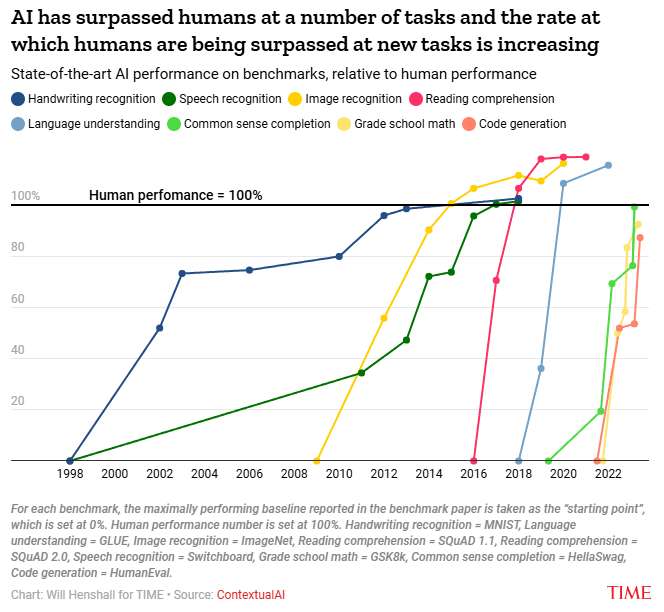
\includegraphics[width=0.75\linewidth]{intelligence.png}
    \caption{Evolución de las inteligencias en distintas habilidades en contraste con el humano.}
    \label{fig:enter-label}
\end{figure}
 
Se menciona el reciente premio nobel de física y química, existe una crítica en relación con la inteligencia artificial pues muchos defienden que cada vez está deshumanizándose este proceso creativo e innovador, en el premio de física uno de los partíciper era neurocientífico lo que no agradó a la audiencia y en química usaron un código para ahorrarse un algoritmo extremadamente pesado de computacionar, por lo que discuten que esta medida de llegar al resultado es impropia de ellos.\\
Se habla como en los discos duros o redes de Hopefield tienden a seguir un patrón final, y el café después de un tiempo de decorarse con leche también llega a un patrón, que si bien para el humano no tiene asociación a ninguna figura o forma pecular es un resultado final muy replicable y lo asocia con el teorema H de Boltzmann.\\

Existen dos proyectos actualmente en méxico: el VLA de nueva generación que es la actualización del sistema de antenas antiguo que recopilará datos del orden de hexabytes. Por otro lado y el más relevante para esta ocasión, el Large Synoptic Survey Telescope, proyecto en el que está trabajando el Dr. Valenzuela, llamado en español "senso del espacio y el tiempo".
Es la cámara más poderosa de la historia de la humanidad del orden de 3,200 millones de pixeles, para poner en situación al lector de este resumen, un teléfono celular tiene una cámara fotográfica que data del orden de 13 megapixeles. Está ubicado en Cerro Pachón, Chile, en principio se quiso poner en México pero el gobierno no quiso participar en proporcionar las medidas adecuadas para establecerlo; lo particular de este telescopio es que con su inteligencia artificial se va adecuando a las situaciones atmosféricas para modificar la estructura de la cámara. 
Se piensa que va a barrer el cielo cada poco menos de 3 días, durante 10 años, se espera observar cada 3 días al rededor de 17 mil millones de estrellas, 20 mil millones de galaxias, NEOS (asteroids), 10 millones de alertas de objetos variables en las que se encuentran: estrellas variables, exoplanetas, asteroides, explosiones de supernova, quasares que varian con el tiempo, choque de agujeros negros, etcétera, y las alertas se despliegan al comparar 30 segundos de muestreo con la información anteriormente interpretada.

A continuación se muestra una comparativa de propiedades asociadas a las estructuras especializadas en la captura del cosmos de los últimos años.
\begin{figure}[h]
    \centering
    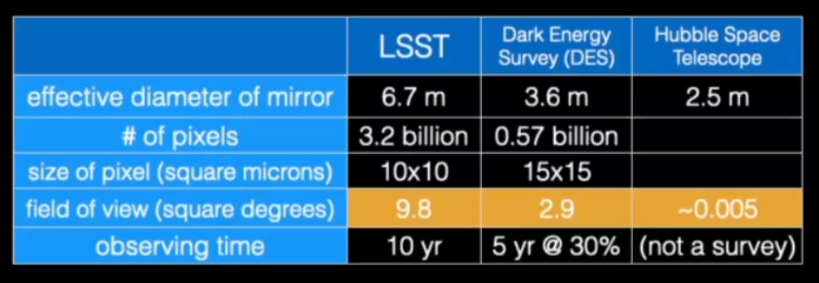
\includegraphics[width=0.5\linewidth]{image2.png}
    \label{fig:enter-label}
\end{figure}

La cámara del LSST tiene un plano de diametro focal de 63cm con 3,200mp, ¿cuántos diplays de Mackbook Retina son requeridos para mostrar solo una foto producida por el LSST en su resolución total? Esta es una pregunta que fue lanzada al público y la respuesta es sorprendente considerando la inmensa calidad de pantalla de este computador, se requieren al menos 600 de estas.\\

En el universo observable se sabe hasta la fecha que existen alrededor de $10^11$ galaxias, volviendo al dato anterior, esta camara puede observar 20 billones, lo cual es una fracción demasiado importante para mejorar estos estudios.
El Dr. Valenzuela comenta que en sus tiempos como estudiante de doctorado sus colegas miraban el telescopio por 3 semanas y solo lograban observar de 10 a 15 galaxias, con lo que ya se podían titular, y eso solo se podía bajo condiciones perfectas porque en lluvia era imposible de verse; con los jóvenes de esta nueva época, los descubrimientos estarán a la alza con una cantidad increíble de datos nueva que nos proporcionaría el LSST gracias a la generación de inteligencias artificiales que está naciendo. Siendo esto el camino para una revolución en la astronomía.\\

Hasta ahora no nos hemos preocupado del manejo de estos datos, y es que la cantidad de información es increíblemente exagerada, por ello se seguirá un modelo similar al CERN: una red internacional de censo de datos conectadas a un ecosistema para distribuir los datos, en lugar de estar en carga y descarga de información se hosteará al usuario que quiere analizar/visualizar cierta rama de datos para que pueda trabajar sobre ella en un servidor específico.\\

Se nos dice que un lente gravitacional es un efecto de curvatura de la luz causado por la gravedad de un objeto masivo, como una galaxia, que actúa como una “lente” al distorsionar y amplificar la luz de objetos detrás de él, como los cuásares (núcleos galácticos activos extremadamente luminosos), permitiendo observarlos a mayores distancias. Bajo estos es posible observar datos muy interesantes con el LSST.\\

Los algoritmos de mapas autoorganizados (SOMs) son redes neuronales que ayudan a analizar datos complejos, útiles en astronomía para clasificar galaxias y cuerpos celestes al organizar grandes cantidades de datos en mapas visuales. En muchas ocasiones para el humano es imposible saber qué es lo que está viendo/recibiendo, si son galaxias muy lejanas, cercanas, supernovas o algun otro cuerpo o conjunto de cuerpos celestes. El machine learning según el Dr. Valenzuela y de forma simple, su principio se basa en la filosofía "si tiene manchas, muge y da leche entonces es una vaca", hacer estas asociaciones nos permite entender lo que estamos viendo en realidad que a simple vista es muy dificil de entender hasta que la inteligencia artificial logra asociar estos patrones dándole las características del cuerpo celeste en donde quizá el mugido sea emitir radiación bajo una frecuencia constante, como un pulsar; con la estructura cósmica que se conoce actualmente se ha ido entrenando a estos algoritmos y cada vez hemos mejorado la hiperresolución de sus imágenes, vemos un ejemplo de como un estudiante de licenciatura gracias a la IA logra simular un fluido bajo las leyes de Navier Stokes con una fluidez y fidelidad muchísimo más alta que computacionándola bajo métodos standard. \\

Nacen preguntas en donde si la inteligencia artificial asistida por el humano al realizar un descubrimiento que computacionalmente es costeable pero el visualizarla experimentalmente es demasiado caro, entonces ¿vale la pena comprobarlo bajo estos métodos clásicos?, en principio parece un dilema facil, pues claramente querrías ahorrarte billones de pesos en un proyecto, pero si se desarrolla algo como un fármaco imposible de poner a prueba bajo métodos clásicos y seguros, ¿vale la pena probarlo directamente en un humano?. Por lo pronto, a pesar de la revolución que está suponiendo la IA, todavía no ha hecho ningún descubrimiento en astronomía, sin embargo, en un futuro no muy lejano en todos los papers de ciencia esta será el pan de cada día.

\end{document}



